\documentclass[letterpaper]{article}
\usepackage{aaai}
\usepackage{times}
\usepackage{helvet}
\usepackage{courier}
\usepackage{graphicx}
\usepackage{amssymb}
\frenchspacing
\pdfinfo{
/Title (Hashing for Lightweight Episodic Recall)
/Subject (AAAI Publications)
/Author (Scott A. Wallace, Evan Dickinson, Andrew Nuxoll)
/Keywords(Episodic Memory,Soar,Reinforcement Learning,Hidden State)
}
\setcounter{secnumdepth}{0}

\begin{document}
\title{Sudoku Solver}
\author{
	Benjamin Longbons\and
    Eric Klinginsmith \and
    Sebastian S\'{a}nchez \\
Washington State University Vancouver \\
14204 NE Salmon Creek Ave. \\
Vancouver, WA 98686
}

\maketitle
\begin{abstract}
This document explores the performance of two separate implementations of Sudoku puzzle agent and the resulting evaluation of the implementations. Each implementation is a distinct search method to solve any Sudoku puzzle. They will be evaluated based on how fast each solves a given set of puzzles. It was our goal to explore these methods to ultimately see how well they worked.
\end{abstract}

\section{Introduction}

A Sudoku puzzle like the one in Figure \ref{fig:sudoku-puzzle} is any $ n^{2} $ by $ n^{2} $ grid sub divided into $ n^{2} $, n by n boxes. In the typical case $ n $ is equal to $3$ which makes the Puzzle a $9$ by $9$ grid with $9$ boxes, each box being it's own $3$ by $3$ grid. In any case, to solve the Puzzle, distinct numbers $1$ through $ n^{2} $ must be filled into every row and column of the grid so that no two numbers are in the same row, column, or box. Our implementations solve any Sudoku puzzle with an $n \not\le 7$.

All of our approaches use partial state.

\section{Terminology}

\emph{Order}: The most basic measure of a puzzle's size, labeled $ n $.

\emph{Grid}: A square 2-dimensional array of Cells. Both dimensions
of the array are $ n^2 $.

\emph{Cell}: A single place that can store a number. In a partial state,
it may also be blank.

\emph{Row}: A horizontal slice of a Grid. It must contain all the
numbers $ 1 $ to $ n^2 $ exactly once.

\emph{Column}: A vertical slice of a Grid. It must contain all the
numbers $ 1 $ to $ n^2 $ exactly once.

\emph{Square}: An aligned $ n \times n $ slice of a Grid. It must contain
all the numbers $ 1 $ to $ n^2 $ exactly once.

\emph{Neighbor} of a Grid: a Grid that differs by adding a value to a
single Cell that previously had no values. The core function in all
solvers is to iterate over all the Neighbors of a Grid at a certain Cell.
For convenience, the Neighbors of a Grid at a Cell that already has a value
is sometimes defined as the same Grid.

\section{Implementations}

\subsection{Stupid Monkey Brains}

\subsubsection{Stupid}
The Stupid Implementation was chosen as a baseline, and simply iterates
over every cell, and recursively checks all Neighbors at that Cell.

It performs terribly when the first Cells visited are relatively
unconstrained and it guesses wrong, but this Implementation \emph{was}
useful to demonstrate the completeness of the general recursive approach.

\subsubsection{Monkey}
The Monkey Implementation was a deliberately naive attempt to improve on
the efficiency of the Monkey, particularly for the worst cases, by
statically ordering the Cells according to their initial neighbor count.

Surprisingly, it actually performed worse in the few tests given to it,
though as both implementations are very slow, it cannot be ruled out that
the difference is just noise.

This implementation also changed the algorithm slightly to skip over
already filled cells.

\subsubsection{Brains}
The Brains Implementation was a serious attempt to continue doing the best
thing as the puzzle iteratively got closer to solved.

It works by calculating, at each step, the number of neighbors at each
yet-unfilled cell, and choosing the one with the least number of
possibilities.

Using this, it achieves pretty good performance for most puzzles. However,
there is still a lot of variation, so it is not yet fully optimized.

\subsubsection{Possible Improvements}
The Brains approach still suffers from two major flaws:

    - It recalculates the list of best nodes every step. It would be better
    to remember a list of most-constrained Cells and update it.

    - It always calculates possible neighbors from $ 1 $ to $ 9 $.
    This will behave badly if larger numbers are more constrained.

Combined, these indicate the reason that certain puzzles take much more
time to solve with this solver compared to the next.


\subsection{SearchNxN Implementation}

The SearchNxN Implementation searches for the solution by filling in one box at a time. To do this, SearchNxN first selects one of the boxes to fill in. Once selected, SearchNxN will generate all possible solutions for the given box. These these solutions are added to a stack. Then for every element on the stack SearchNxN selects the next box to fill in. This process is repeated until either all boxes are filled in, or the stack is empty. If all boxes are filled in, then the solution is printed to stdout. Otherwise, there is no solution and \emph{false} is returned. The inspiration behind this method was taken from the common computer science problem of a three coloring. A three coloring is a problem in which when given a map with $n$ regions to color an agent finds a way to color the entire map with only three colors so that no two regions have the same two colors. If we think of the Sudoku puzzle as being a map where no two numbers can be in the same row, column, or box and each box is a region, then a so called three coloring of a Sudoku puzzle would be to "color" each box so that there are no violations where a color would be one of the possible solutions to that box.

\begin{figure}[h]
	\centering
	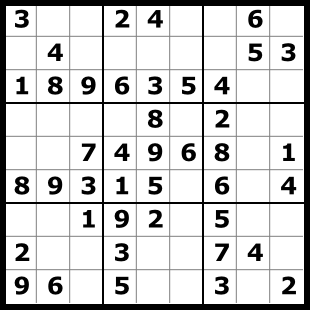
\includegraphics[width=60mm]{./Sudoku-games.png}
	\caption{Sudoku Puzzle}
	\label{fig:sudoku-puzzle}
\end{figure}

\subsection{About sole candidates}

We would like to mention one other part to our implementation. This is the idea of sole candidates. In a Sudoku puzzle, there are sometimes cells where only one number can be placed there. This means that any partially solved puzzle can have one or more sole candidates. If a sole candidate is found, then our implementation will try to find another. This continues until either all the sole candidates have been found, or it hits a cell where there are no possibilities. If the result is the latter, then that branch of the search is invalid and therefore the search must then try a different path to find the solution. If there are no other branches to explore and a solution has not been found then there is no solution to the given puzzle.

\section{Experiments\newline}

\subsection{SearchNxN Performance}

Now lets look at the performance of the SearchNxN implementation.There are several different ways we measured the performance of the SearchNxN implementation.

\begin{figure}[h]
    \centering
    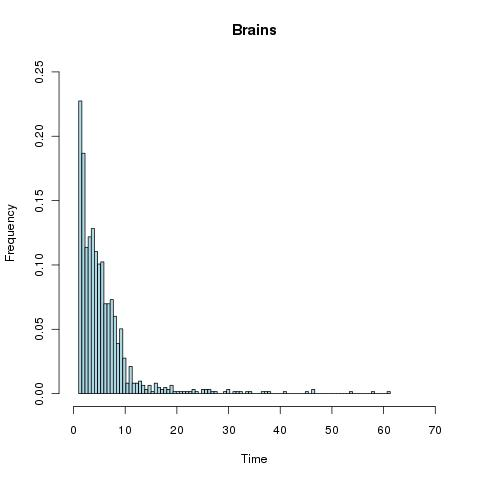
\includegraphics[width=60mm]{./brains_stats.jpg}
    \caption{Histogram for Brains Strategy}
    \label{fig:brains-strategy}
\end{figure}

\begin{tabular}{|l|l|l|l|l|l|}
\hline
Min. & 1st Qu.  & Median & Mean & 3rd Qu. & Max.\\
\hline
1.008 & 2.212 & 4.298 & 5.844 & 7.095 & 61.290\\
\hline
\end{tabular}

\subsection{Brains Performance}

\subsubsection{Comparing the two}

\section{Conclusions}

\end{document}